%----------------------------------------------------------------------------------------
%
% LaTeX-template for degree projects at LNU, Department of Computer Science
% Last updated by Johan Hagelbäck, Oct 2015
% Linnaeus University
%
% License: Creative Commons BY
%
%----------------------------------------------------------------------------------------

%----------------------------------------------------------------------------------------
%	Settings and configuration
%----------------------------------------------------------------------------------------

\documentclass[a4paper,12pt]{article}
\usepackage[T1]{fontenc}
\usepackage{times}
\usepackage[english]{babel}
\usepackage[utf8]{inputenc}
\usepackage{caption}
\usepackage{subcaption}
\usepackage{wallpaper}
\usepackage[absolute]{textpos}
\usepackage[top=2cm, bottom=2.5cm, left=3cm, right=3cm]{geometry}
\usepackage{appendix}
\usepackage[nottoc]{tocbibind}
\usepackage[hidelinks]{hyperref}
\setcounter{figure}{0}
%\setcounter{secnumdepth}{3}
%\setcounter{tocdepth}{3}
\usepackage{amsmath}
\numberwithin{figure}{section}
\usepackage{sectsty}
\sectionfont{\fontsize{14}{15}\selectfont}
\subsectionfont{\fontsize{12}{15}\selectfont}
\subsubsectionfont{\fontsize{12}{15}\selectfont}

\usepackage{csquotes} % Used to handle citations

\renewcommand{\thetable}{\arabic{section}.\arabic{table}}  
\renewcommand{\thefigure}{\arabic{section}.\arabic{figure}} 

%----------------------------------------------------------------------------------------
%	
%----------------------------------------------------------------------------------------
\newsavebox{\mybox}
\newlength{\mydepth}
\newlength{\myheight}

\newenvironment{sidebar}%
{\begin{lrbox}{\mybox}\begin{minipage}{\textwidth}}%
{\end{minipage}\end{lrbox}%
 \settodepth{\mydepth}{\usebox{\mybox}}%
 \settoheight{\myheight}{\usebox{\mybox}}%
 \addtolength{\myheight}{\mydepth}%
 \noindent\makebox[0pt]{\hspace{-20pt}\rule[-\mydepth]{1pt}{\myheight}}%
 \usebox{\mybox}}

%----------------------------------------------------------------------------------------
%	Title section
%----------------------------------------------------------------------------------------
\newcommand\BackgroundPic{
    \put(-2,-3){
    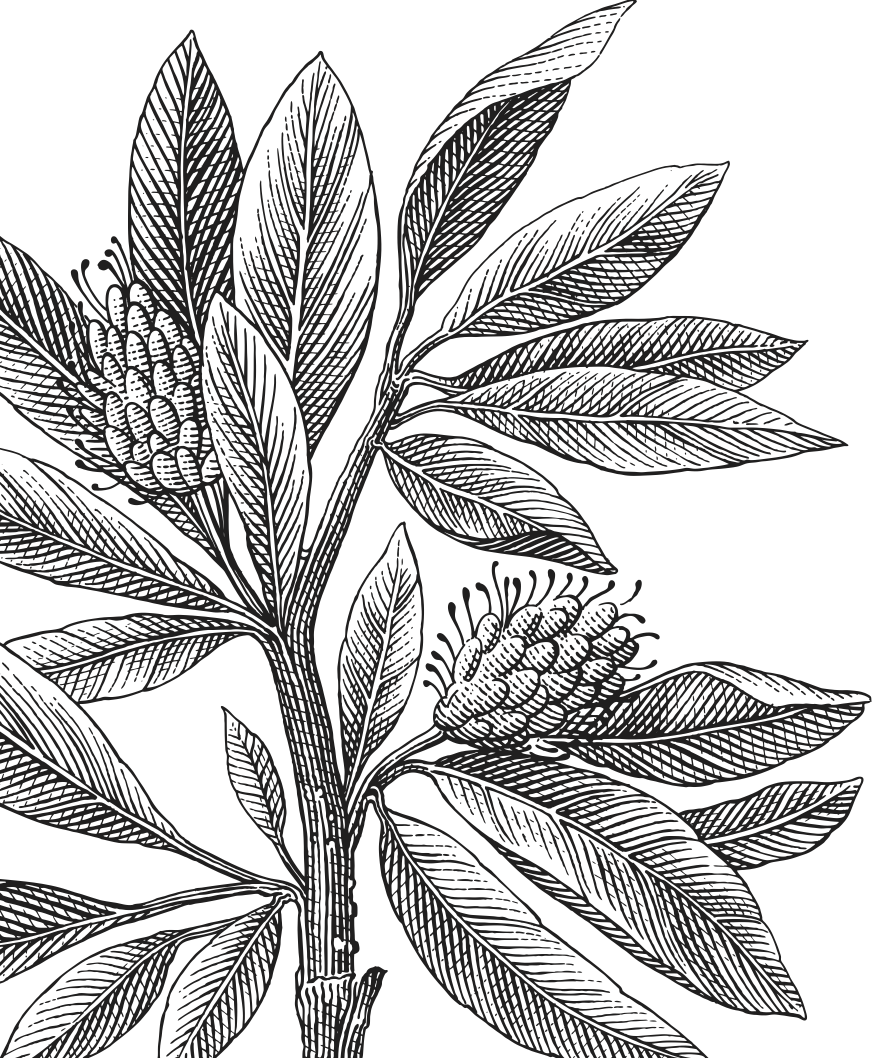
\includegraphics[keepaspectratio,scale=0.3]{img/lnu_etch.png} % Background picture
    }
}
\newcommand\BackgroundPicLogo{
    \put(30,740){
    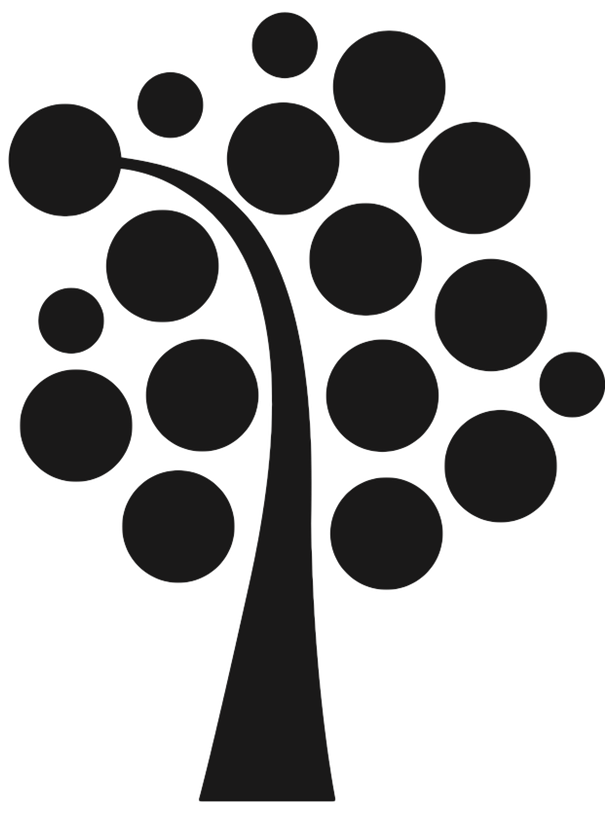
\includegraphics[keepaspectratio,scale=0.10]{img/logo.png} % Logo in upper left corner
    }
}

\title{	
\vspace{-8cm}
\begin{sidebar}
    \vspace{10cm}
    \normalfont \normalsize
    %\Huge Bachelor/Master Thesis Project \\
    \vspace{-1.3cm}
\end{sidebar}
\vspace{3cm}
\begin{flushleft}
    \huge Computer networks - 1DV701 \\ 
    \LARGE  Assignment 1\\
\end{flushleft}
\null
\vfill
\begin{textblock}{6}(10,13)
\begin{flushright}
\begin{minipage}{\textwidth}
\begin{flushleft} \large
\emph{Author:} Michael Johansson\\ % Author
%\emph{Supervisor:} Name of your supervisor\\ % Supervisor
%\emph{Examiner:} Dr.~Mark \textsc{Brown}\\ % Examiner (course manager)
\emph{Semester:} VT 2017\\ % 
%\emph{Subject:} Computer Science\\ % Subject area
\end{flushleft}
\end{minipage}
\end{flushright}
\end{textblock}
}

\date{} 

\begin{document}
\pagenumbering{gobble}
\newgeometry{left=5cm}
\AddToShipoutPicture*{\BackgroundPic}
\AddToShipoutPicture*{\BackgroundPicLogo}
\maketitle
\restoregeometry
\clearpage


%----------------------------------------------------------------------------------------
\newpage
\pagenumbering{gobble}
\tableofcontents % Table of contents
\newpage
\pagenumbering{arabic}

%----------------------------------------------------------------------------------------
%
%	Here follows the actual text contents of the report.
%
%----------------------------------------------------------------------------------------

\section{Problem one}

\begin{figure}[h!]
	\centering
	\label{ping}
	\includegraphics[width=0.95\textwidth,keepaspectratio]{img/problem_1_ping.jpg} % first figure itself
	\caption{Pinging host machine inside virtual network 192.168.56.0/24}
\end{figure}

\newpage

\section{Problem two}

\begin{figure}[h!]
	\centering
	\includegraphics[width=0.95\textwidth,keepaspectratio]{img/problem_2_send_5.jpg}
	\caption{Sending 5 UDP packets}
	\label{send5} 

\end{figure}

\subsection{List of handled exceptions}

\begin{itemize}
	\item \textbf{Exceptions in Java library}
	\begin{enumerate}
		\item\textbf{IOException}: Occurs when there is a failure to write/read to our packets or streams.
		\item \textbf{NumberFormatException}: Occurs when there is a failure to parse a string to an Integer.
		\item \textbf{InterruptedException}: Occurs if another thread interrupts our current thread.
	\end{enumerate}
	\item \textbf{Created exceptions}
		\begin{enumerate}
			\item\textbf{NotCorrecctNumberOfArgumentsException}: Occurs when there is less or more then 4 program arguments.
			\item \textbf{NotACorrectIPv4AddressException}: Occurs when the ip address arguments is not "localhost", 4 octants long or has numbers less that zero or more than 255 in an octant.
			\item \textbf{NotCorrectPortNumberException}: Occurs when the port number argument is less than 1024 \cite{portNumbers}. Or more than a 16 bit Integer(65535).
			\item \textbf{ NegativeBufferSizeException}: Occurs if the buffer size argument is less then zero
			\item \textbf{NegativeTransferRateException}: Occurs if the transfer rate argument is less the zero.
		\end{enumerate}
\end{itemize}

\subsection{VG 1, X nr of packets/second}

My solution here is that i check a average time of what the code takes to run and then check if were still inside the simulation time if we sleep for our wait time plus our average time. If that would take us outside the simulation time we just sleep until we reached that time. Else we sleep for our calculated wait time.
As i show in figure \ref{send5} we can se that when i send 5 packets, we get a time taken of 1000 ms. And in figure \ref{VG} we can se that if we have packets left after 1 second we display how many that wasn't sent.

\begin{figure}[h!]
	\centering
	\includegraphics[width=0.95\textwidth,keepaspectratio]{img/VG_1.jpg} 
	\caption{Sending 1000 UDP packets, stop sending at 1 second, 684 packets left to send.}
	\label{VG}
\end{figure}

\subsection{VG 2, NetworkLayer abstract}

I have created an abstract class networkLayer that has the functions which check if our arguments is correct. It also holds our fields that are the same for both UDP and TCP implementations. See \cite{myFiles}.

\begin{figure}[h!]
	\centering
	\includegraphics[width=0.95\textwidth,keepaspectratio]{img/NetworkLayer.jpg} 
	\caption{Top of abstract networking layer class}
	\label{layer}
\end{figure}

\newpage

\section{Problem three}

Server handles multi client as my server creates a new ClientThread for each socket it accepts though the ServerSocket. This ClientThread object has all the code for echo and also handles that we read until buffer is empty. 

This ClientThread have also a time out time as of now 1.5 seconds that if the client dont send anything for that period we close the socket.

As figure \ref{clients} show we have 5 clients connected at once running on different threads. 
I set a simulation time of 10 seconds instead of one as i cant be so quick starting clients that we have two running simultaneous.

\begin{figure}[h!]
	\centering
	\includegraphics[width=0.95\textwidth,keepaspectratio]{img/Many_clients.jpg} 
	\caption{Showing multi client connections}
	\label{clients}
\end{figure}

\subsection{TCP/UDP buffer comparison} 

\begin{itemize}
	\item \textbf{UDP} If we have a smaller buffer then message we only get buffer size of the message and discard the rest of the UDP packet. So as we see in figure \ref{UDPsmall} we get the first 5 bytes in every packet as we have buffer size 5. 
	
	\item \textbf{TCP} Here if we have a smaller buffer then message and only read from the stream one each message sent we get as figure \ref{TCPsmall}. We cant discard those bytes left in the stream as we do when we read from packets in UDP. Here we read 5 bytes from the stream each time and even if we sent 5 full length messages we only read 5 bytes of the stream each time. 
\end{itemize}

\begin{figure}[!h]
	\centering
	\begin{minipage}{.5\textwidth}
		\centering
		\includegraphics[width=\linewidth]{img/UDPsmallbuffer.jpg}
		\captionof{figure}{How UDP handle buffer size 5}
		\label{UDPsmall}
	\end{minipage}%
	\begin{minipage}{.5\textwidth}
		\centering
		\includegraphics[width=0.9\linewidth]{img/TCPsmallbuffer.jpg}
		\captionof{figure}{How TCP handle buffer size 5}
		\label{TCPsmall}
	\end{minipage}
\end{figure}

\newpage

\section{Problem four}

I came across this virtual network card bug where it only capture traffic from my server to client not what my client sent. This we se because we only have traffic from server(IP 192.168.56.101:4950) to client(IP 192.168.56.1:58807).

But what we see in figure \ref{UDPwire} is that first we have an ARP request that tells my client where my server is on the network though the MAC address, as we are inside the network. Then we see that the server sends back packets with the length of Data is 16 bytes(An Echo Message!). As UDP has no reliability this is all we get.  


\begin{figure}[h!]
	\centering
	\includegraphics[width=0.95\textwidth,keepaspectratio]{img/UDPwire.jpg} 
	\caption{Showing Wireshark capturing UDP traffic}
	\label{UDPwire}
\end{figure}

\noindent Then we have the TCP capture. In figure \ref{TCPwire} we still have the problem with just seeing server to client communication. First we dont see the SYN(Synchronize) that the client send to the server to connect to it. But we can see that the server responds to that SYN by the server sending an SYN-ACK(Synchronize acknowledgment) where it updates the sequence number by one. Then the PSH is that the server says to the client that is should not wait for anymore packets and send data that is buffered up to the application that uses it. 

\begin{figure}[h!]
	\centering
	\includegraphics[width=0.95\textwidth,keepaspectratio]{img/TCPwire.jpg} 
	\caption{Showing Wireshark capturing TCP traffic}
	\label{TCPwire}
\end{figure}

\subsection{Difference in wireshark, UDP vs TCP}

The difference here is only that TCP has more reliability because it has all this flags with ACK and SYN. UDP is more fire and forget and if it arrives we cant know for sure. 

The buffer sizes we cant see any difference on here as this all happens in the reading face of the client. So we are always sending the full message.  

\newpage
\bibliographystyle{IEEEtran}
\bibliography{reference}
\end{document}
